
\subsection{Simulation Example}
\begin{frame}{Setup}
Simulate the $\textrm{AR}(1)$ process $X_t = 0.9 X_{t-1} + Z_t$.
\begin{itemize}
    \item
    Innovations $\{Z_t\} \iid \dist{U}(-\sqrt{3}, \sqrt{3})$ are
    mean 0, variance 1 white noise.

    \item
    Draw $64$ observations.

    \item
    Recall that $\hat{\rho}(1)$ is the Yule-Walker estimate for the
    AR parameter~$0.9$.

\end{itemize}
\end{frame}

\begin{frame}{Series Plot}
    \begin{figure}
    \centering
    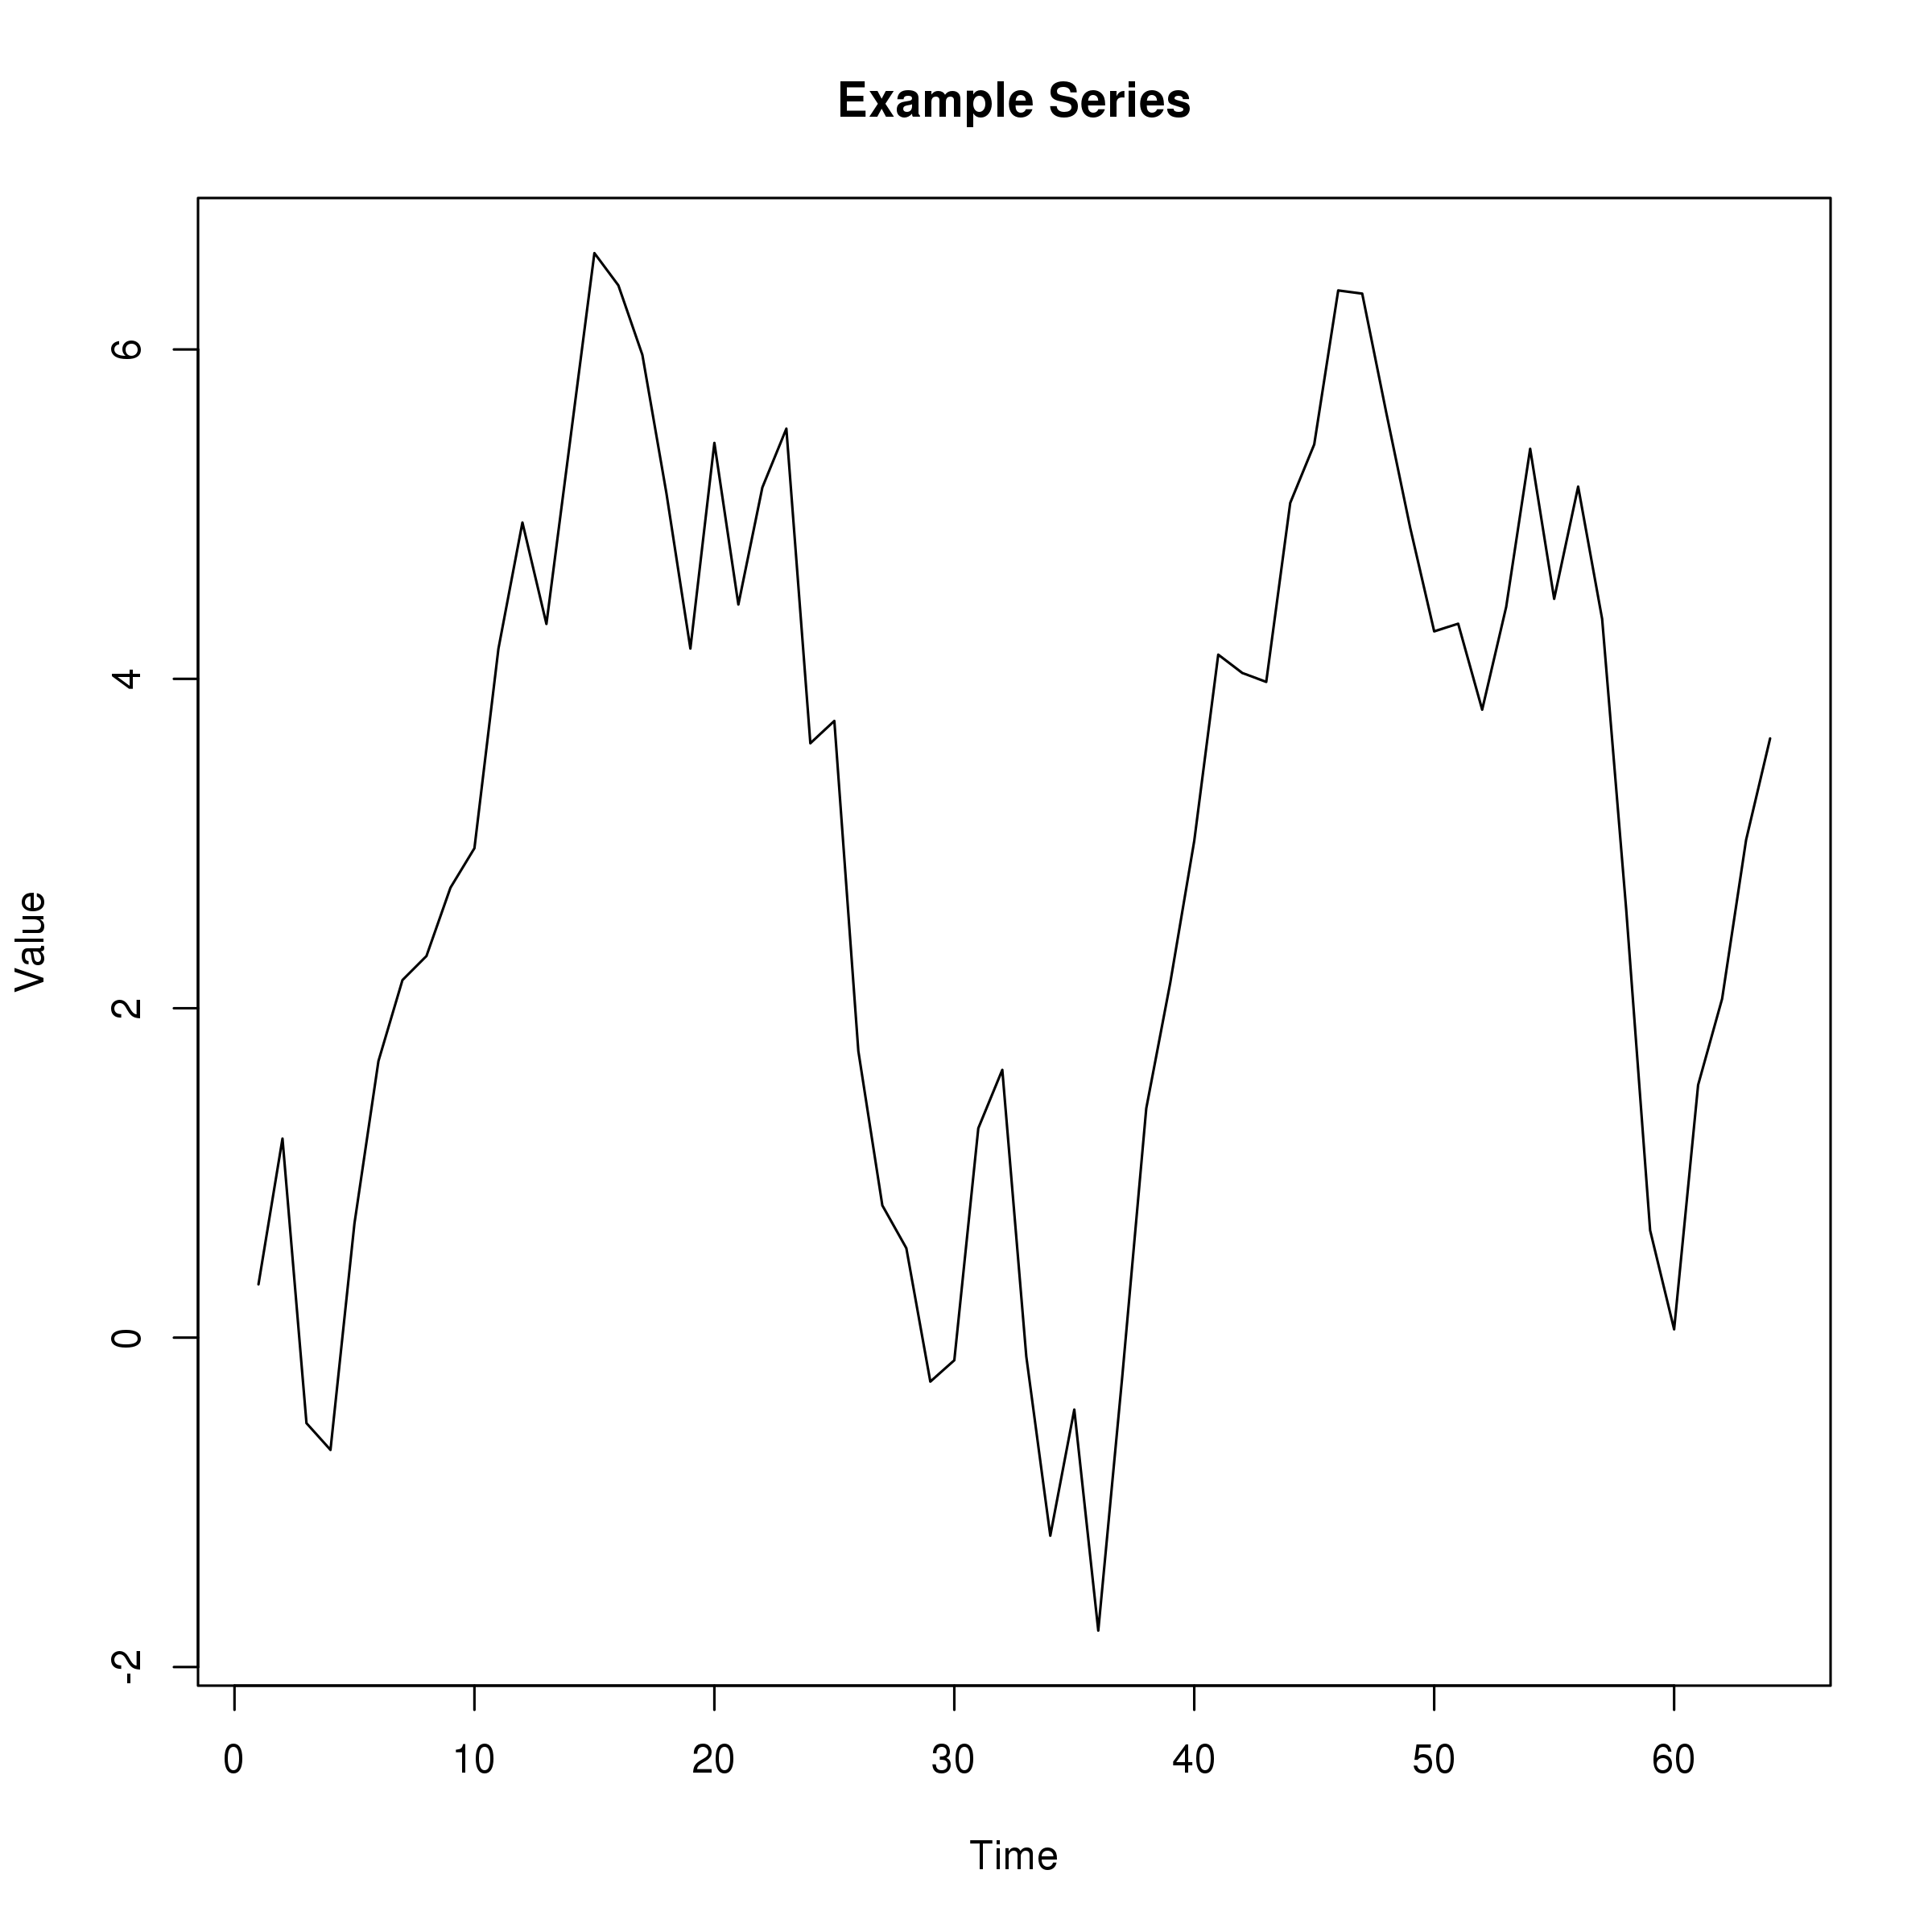
\includegraphics[width = 0.95\textwidth]{res/ex1.png}
    \end{figure}
\end{frame}

\begin{frame}{Practical Details}
\begin{itemize}
    \item
    Computed the periodogram with a $10\%$ Tukey-Hanning taper.
    \item
    Smoothed the log-periodogram using the Epanechnikov kernel
        \[
        K(x) 
        = 
        \frac{3}{4}\pi \biggl[ 1 - \Bigl( \frac{x}{\pi} \Bigr)^2 \biggr].
        \]
    and bandwidth $0.1$ to obtain an estimate of the spectral density.
\end{itemize}
\end{frame}

% Include plots of the Tukey-Hanning taper and the Epanechnikov kernel.

\begin{frame}{Error Distribution}
\begin{itemize}
    \item
    Since $\hat{\rho}(1)$ is the Yule-Walker estimate for the AR parameter,
    then as $n \to \infty$,
        \[
        \sqrt{n} \biggl( \frac{\hat{\rho}(1) - 0.9}{\sqrt{c}} \biggr)
        \inD
        \dist{N}(0, 1 - 0.9^2),
        \]
    where $c$ is a correction for the taper.

    \item
    $2000$ bootstrapped estimates (from one simulation)
    produce a bootstrapped distribution.

    \item
    2000 simulations approximate the true distribution.
\end{itemize}
\end{frame}

\begin{frame}{Distributions Plot}
    \begin{figure}
    \centering
    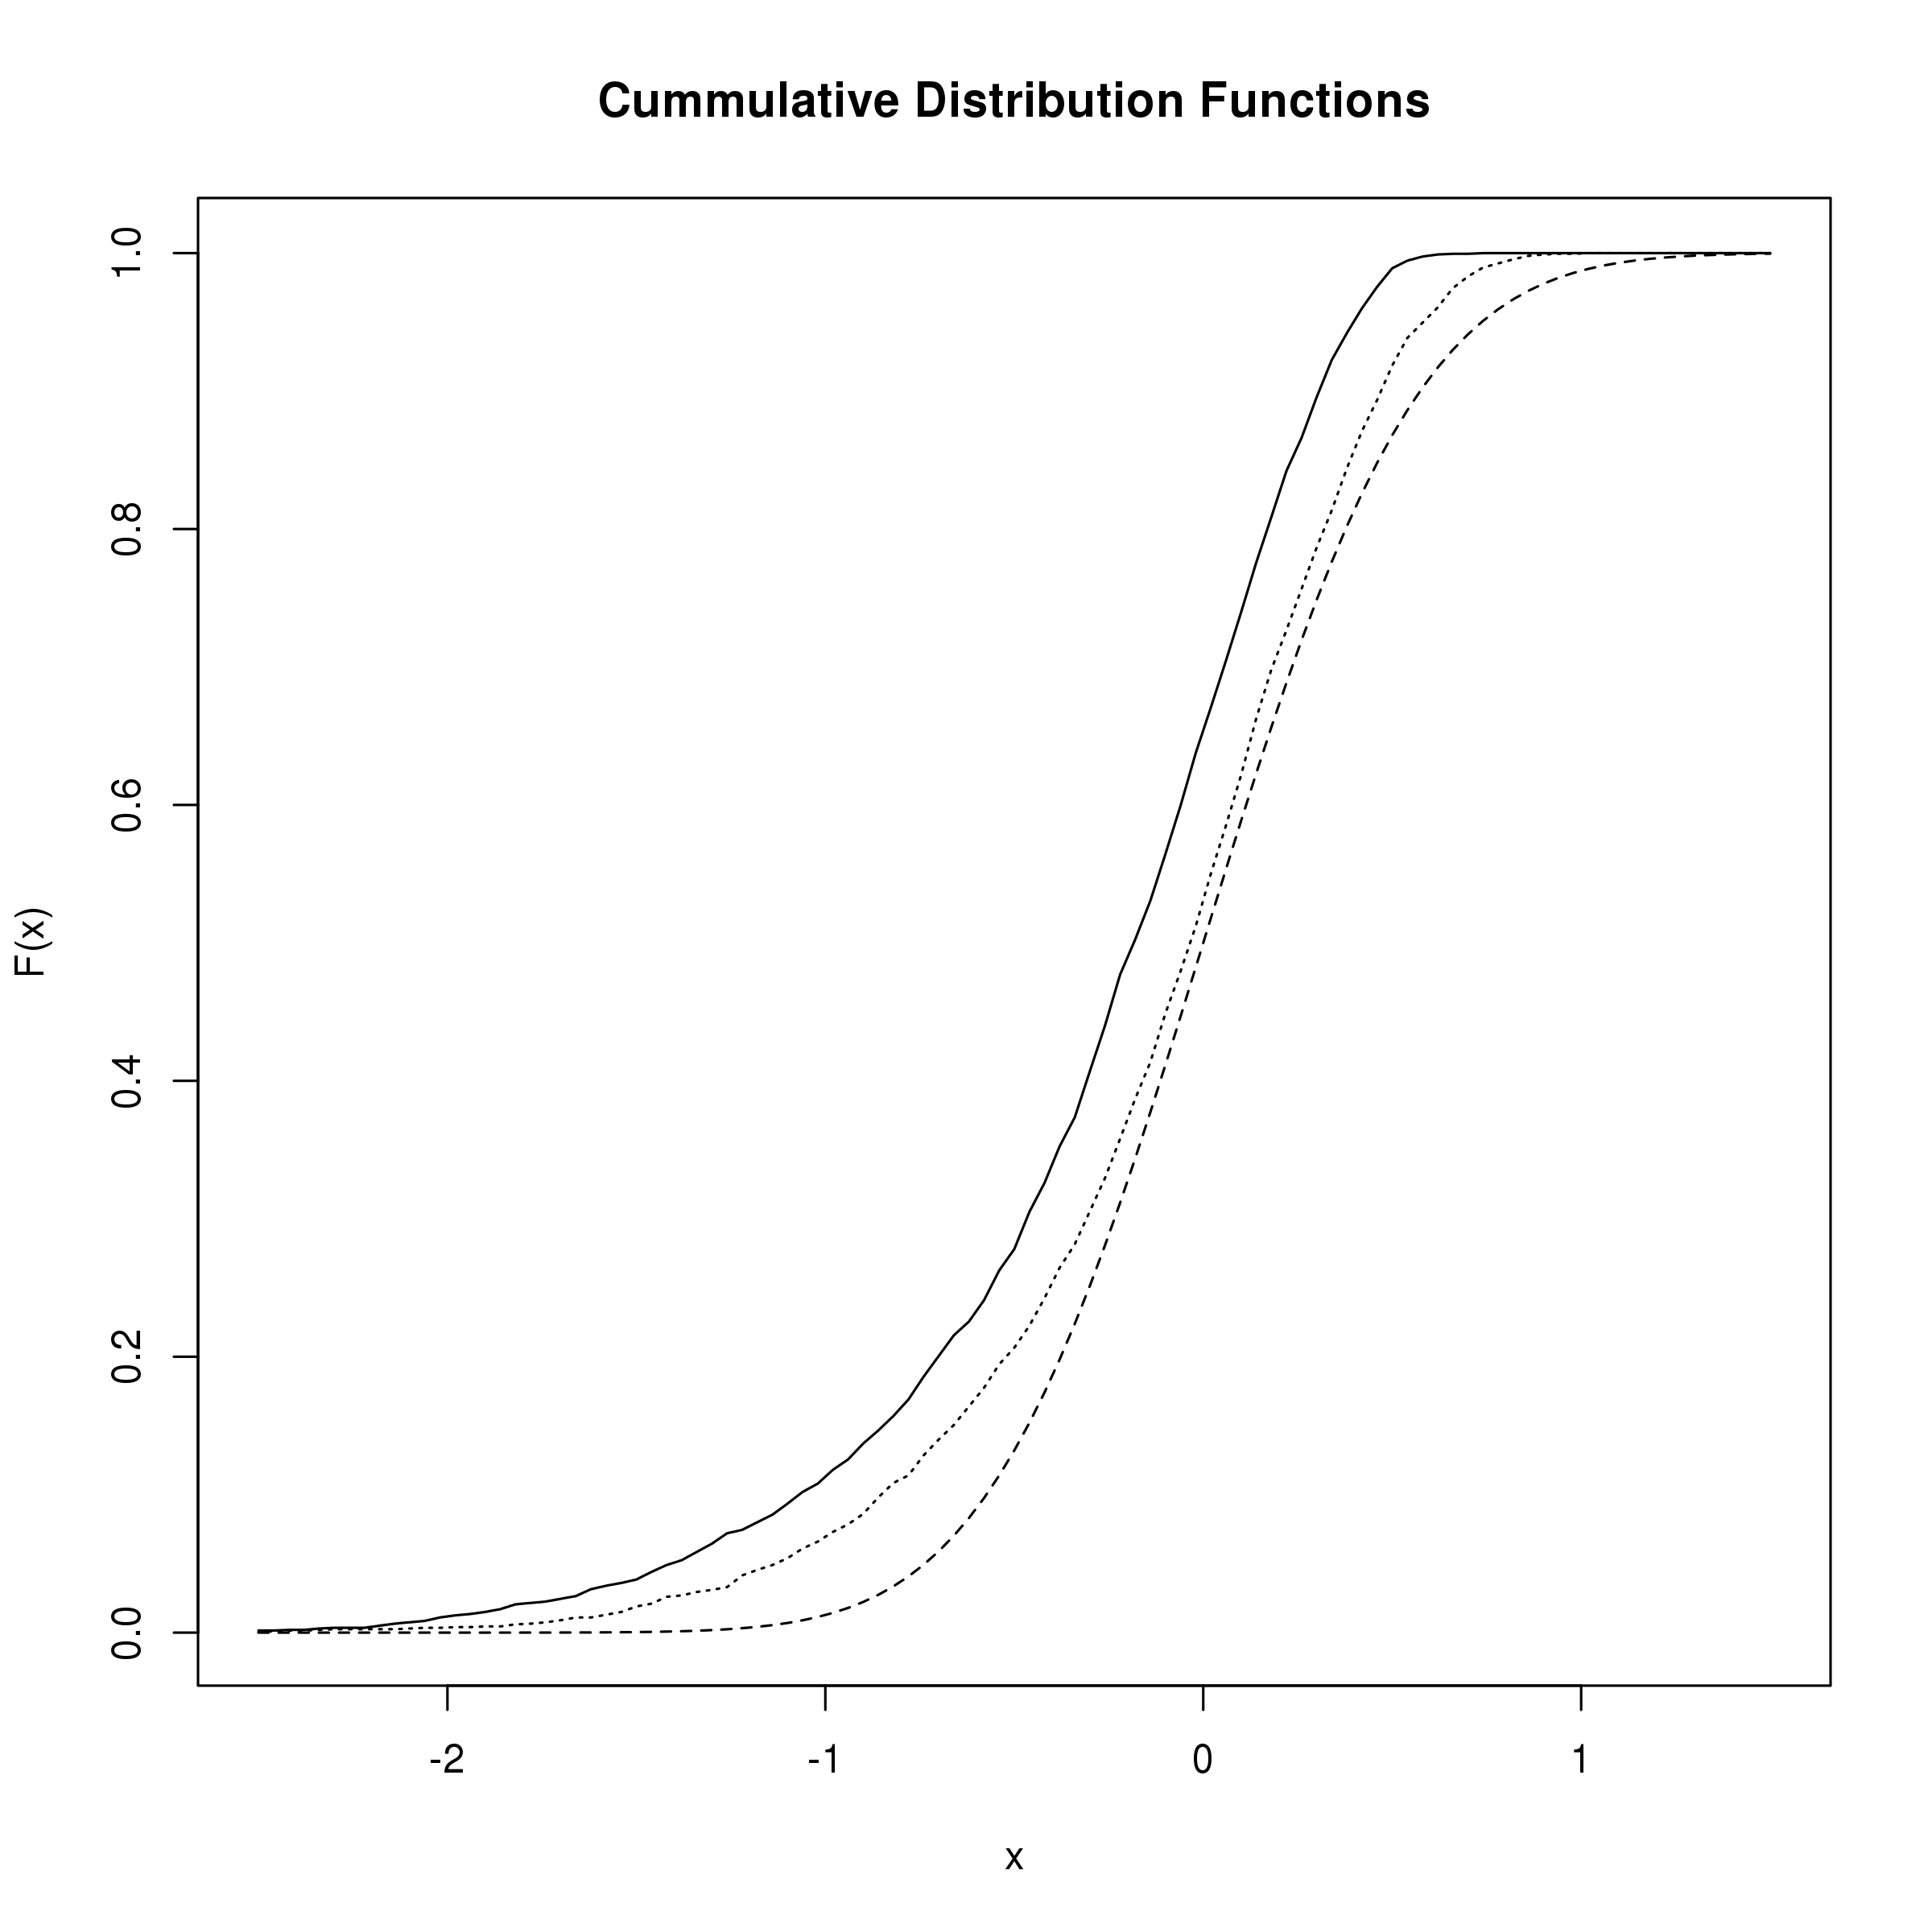
\includegraphics[width = 0.95\textwidth]{res/ex1_cdf.png}
    \end{figure}
\end{frame}

\subsection{Applied Example}
\begin{frame}{Series Plot}
    \begin{figure}
    \centering
    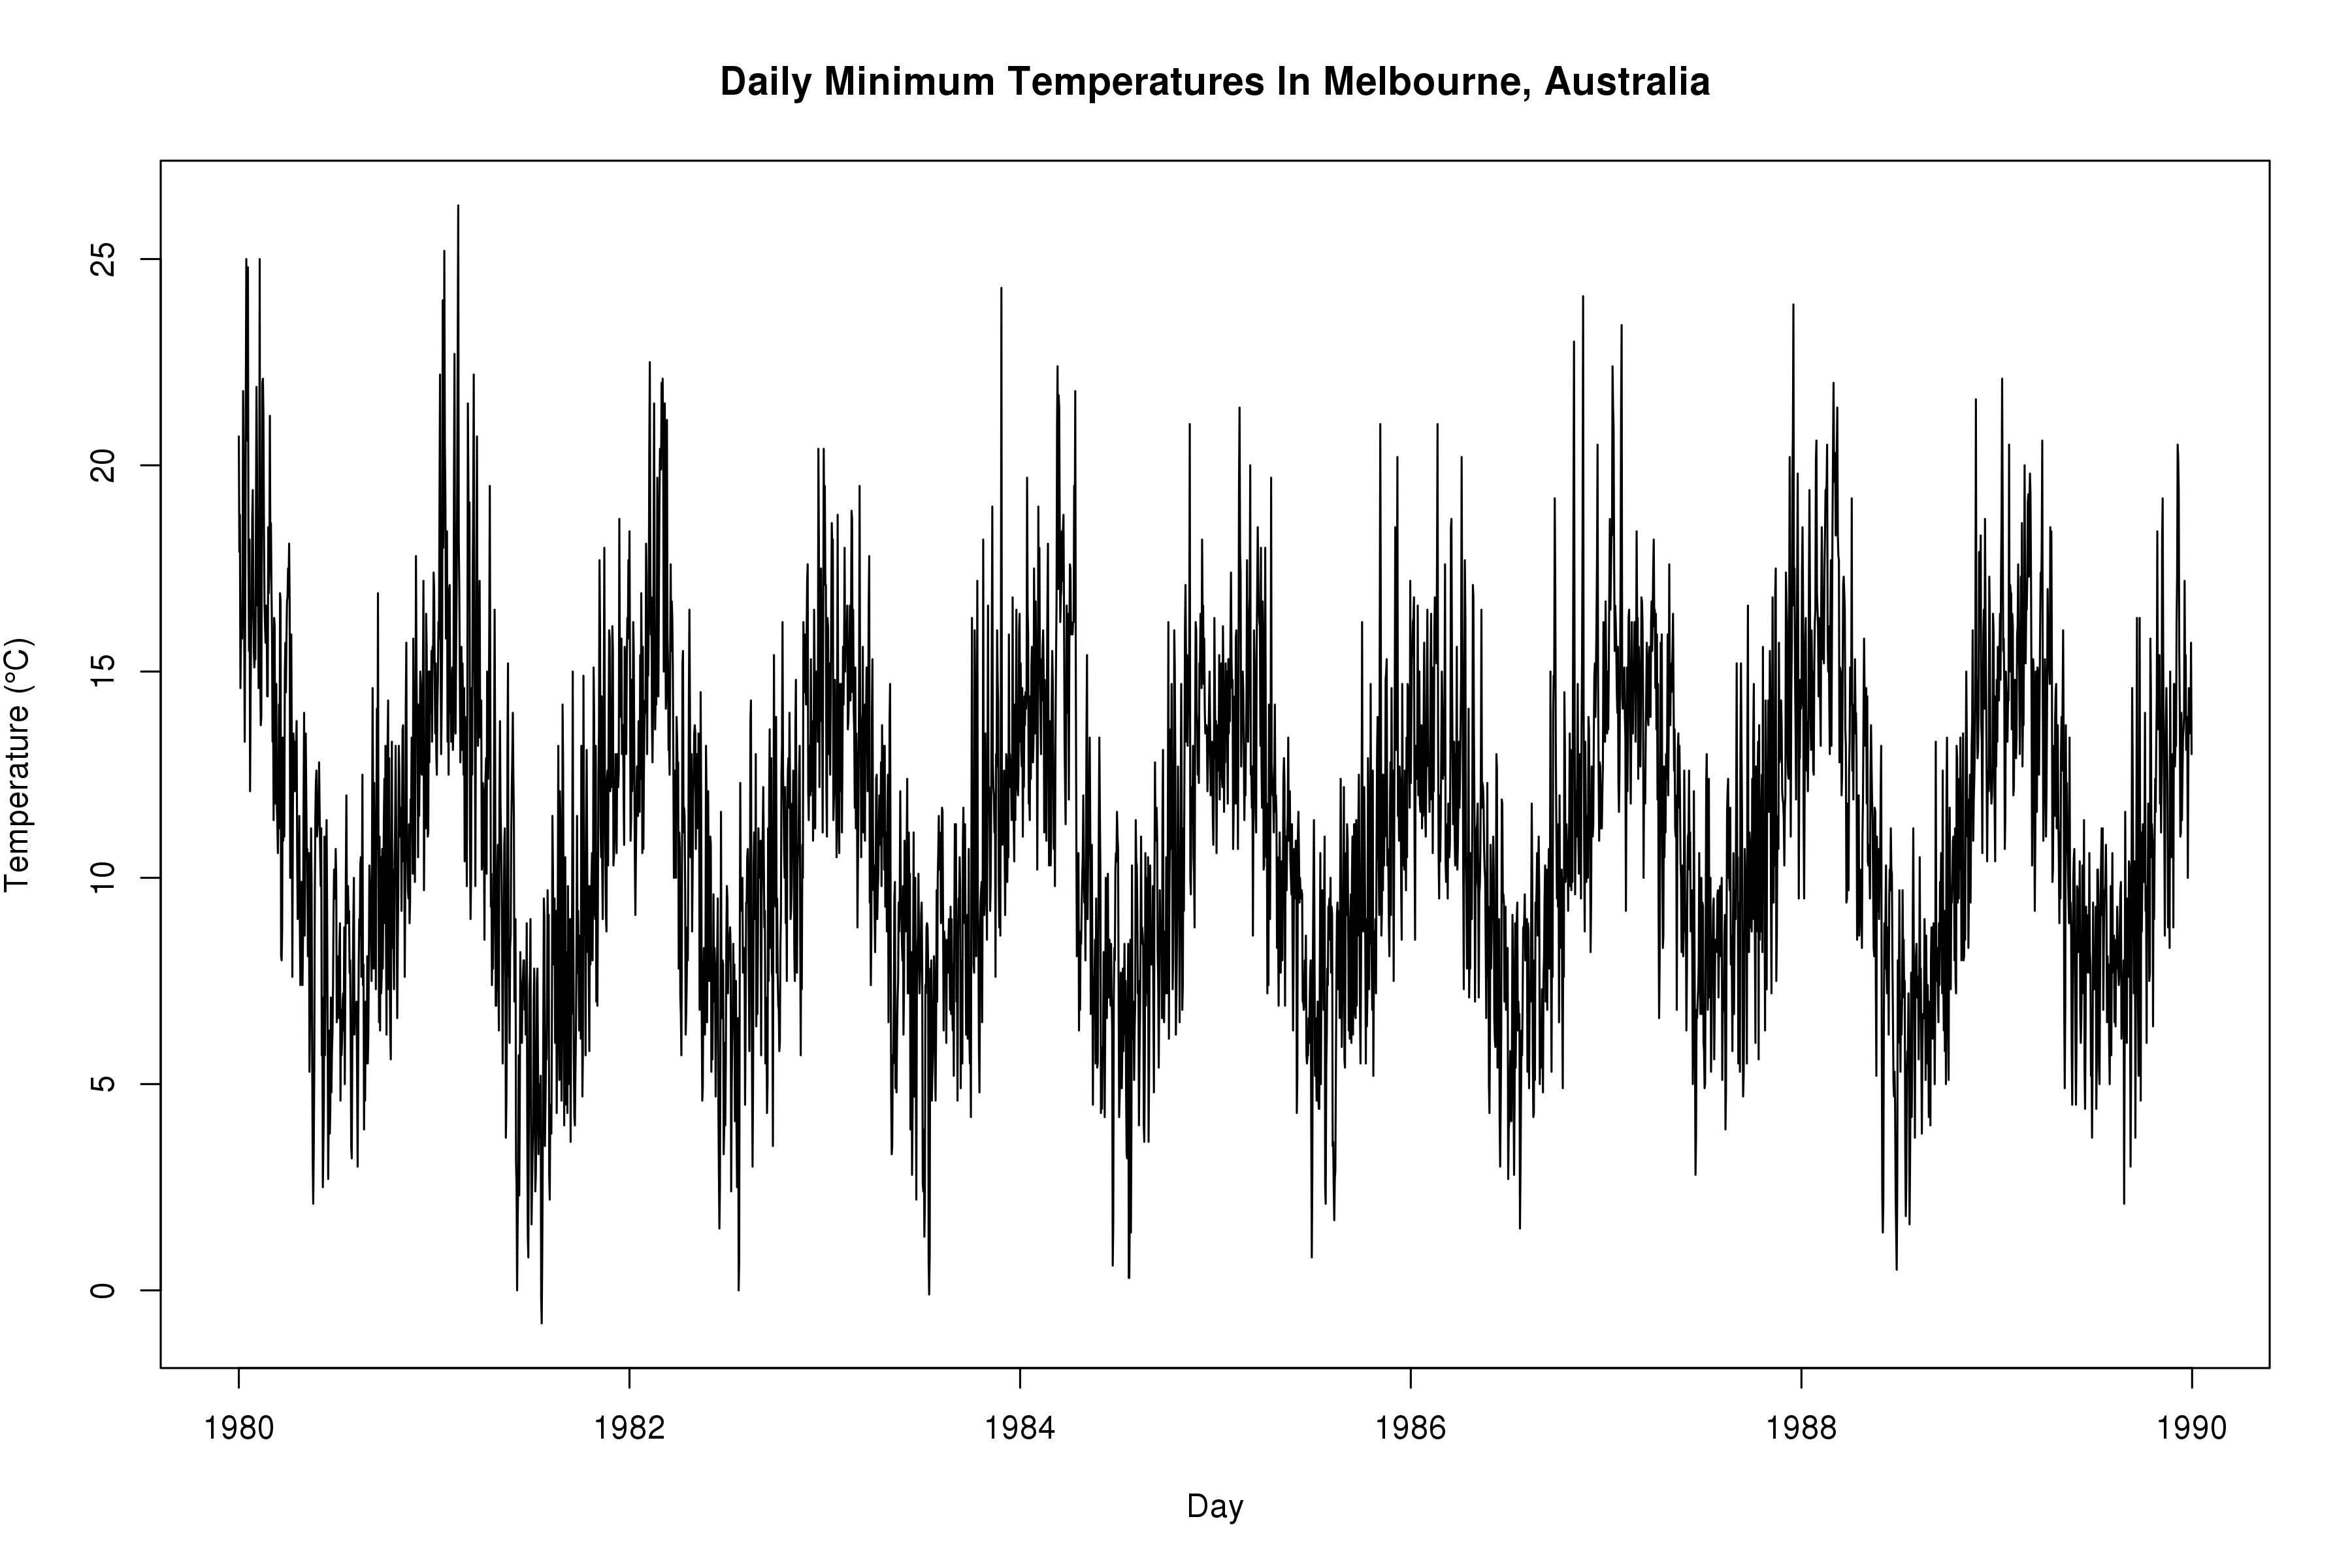
\includegraphics[width = 0.95\textwidth]{res/exA.png}
    \end{figure}
\end{frame}

\begin{frame}{Spectral Density Estimate}
    \begin{figure}
    \centering
    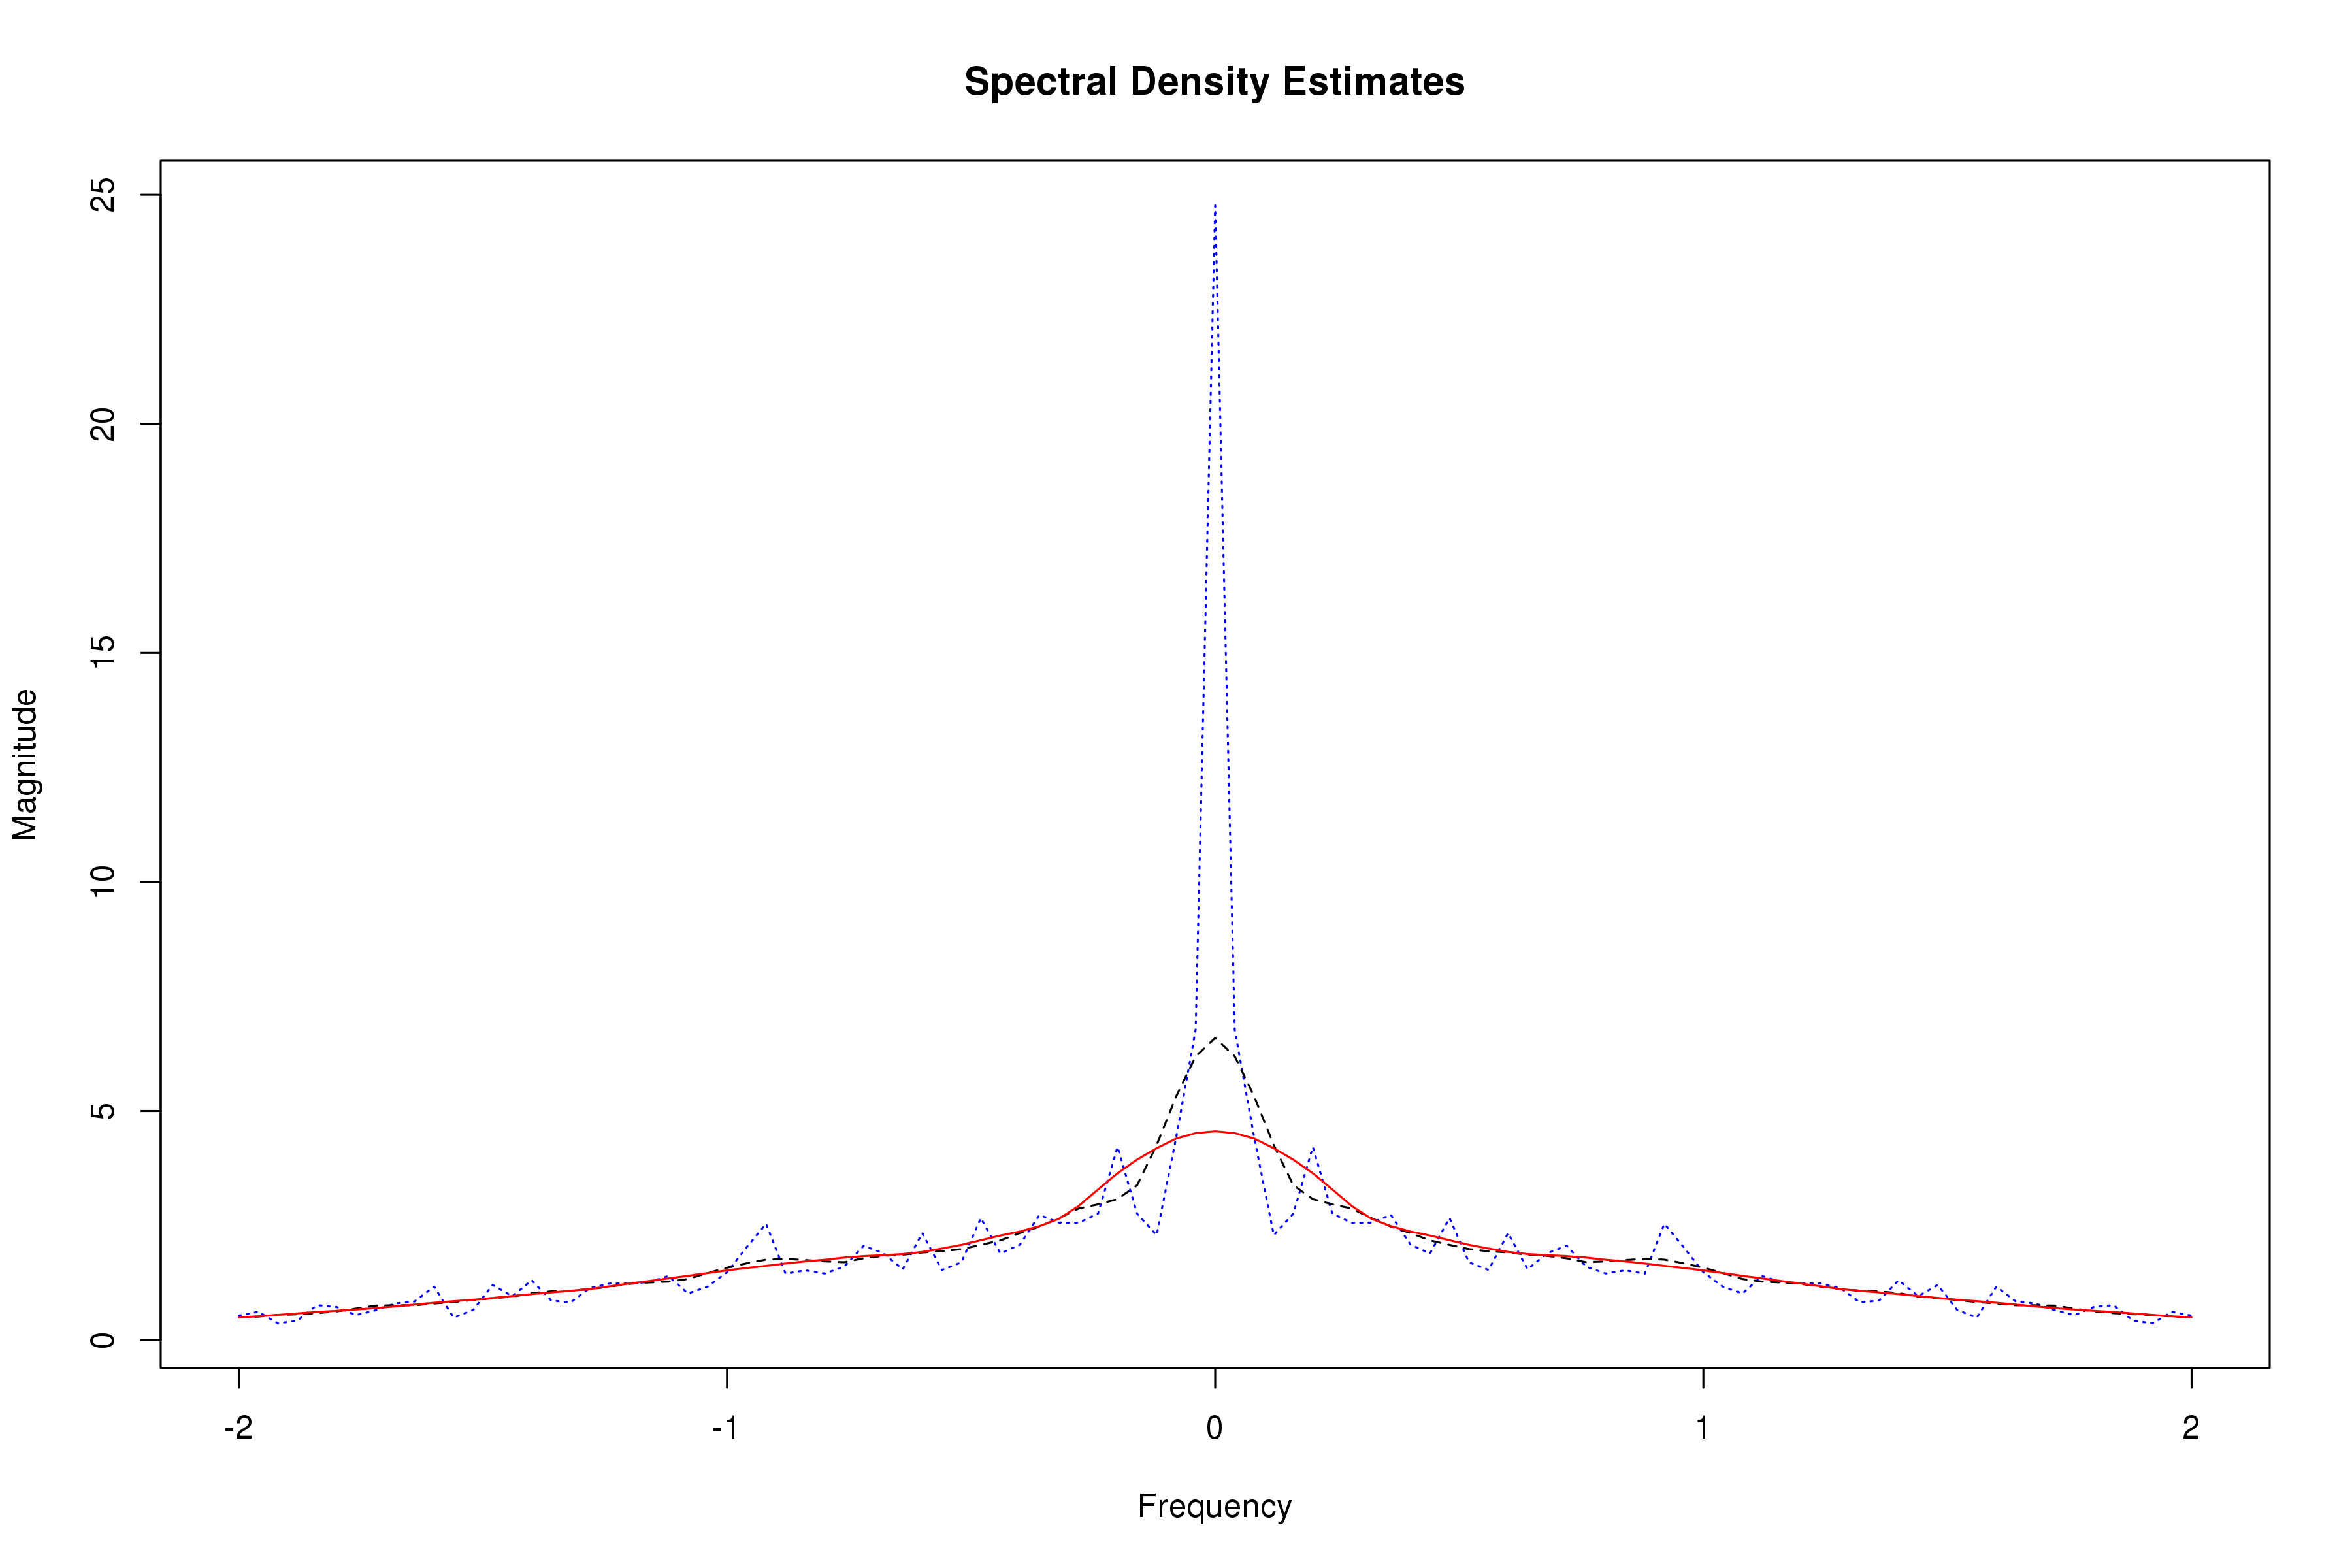
\includegraphics[width = 0.95\textwidth]{res/exA_spec.png}
    \end{figure}
\end{frame}

\begin{frame}{Autocorrelation Estimates}
    \begin{itemize}
    \item
    Lag-1 autocorrelation confidence interval $(0.5234, 0.5787)$.

    \item
    Lag-2 autocorrelation confidence interval $(0.2041, 0.2917)$.
    \end{itemize}

    \begin{figure}
    \centering
    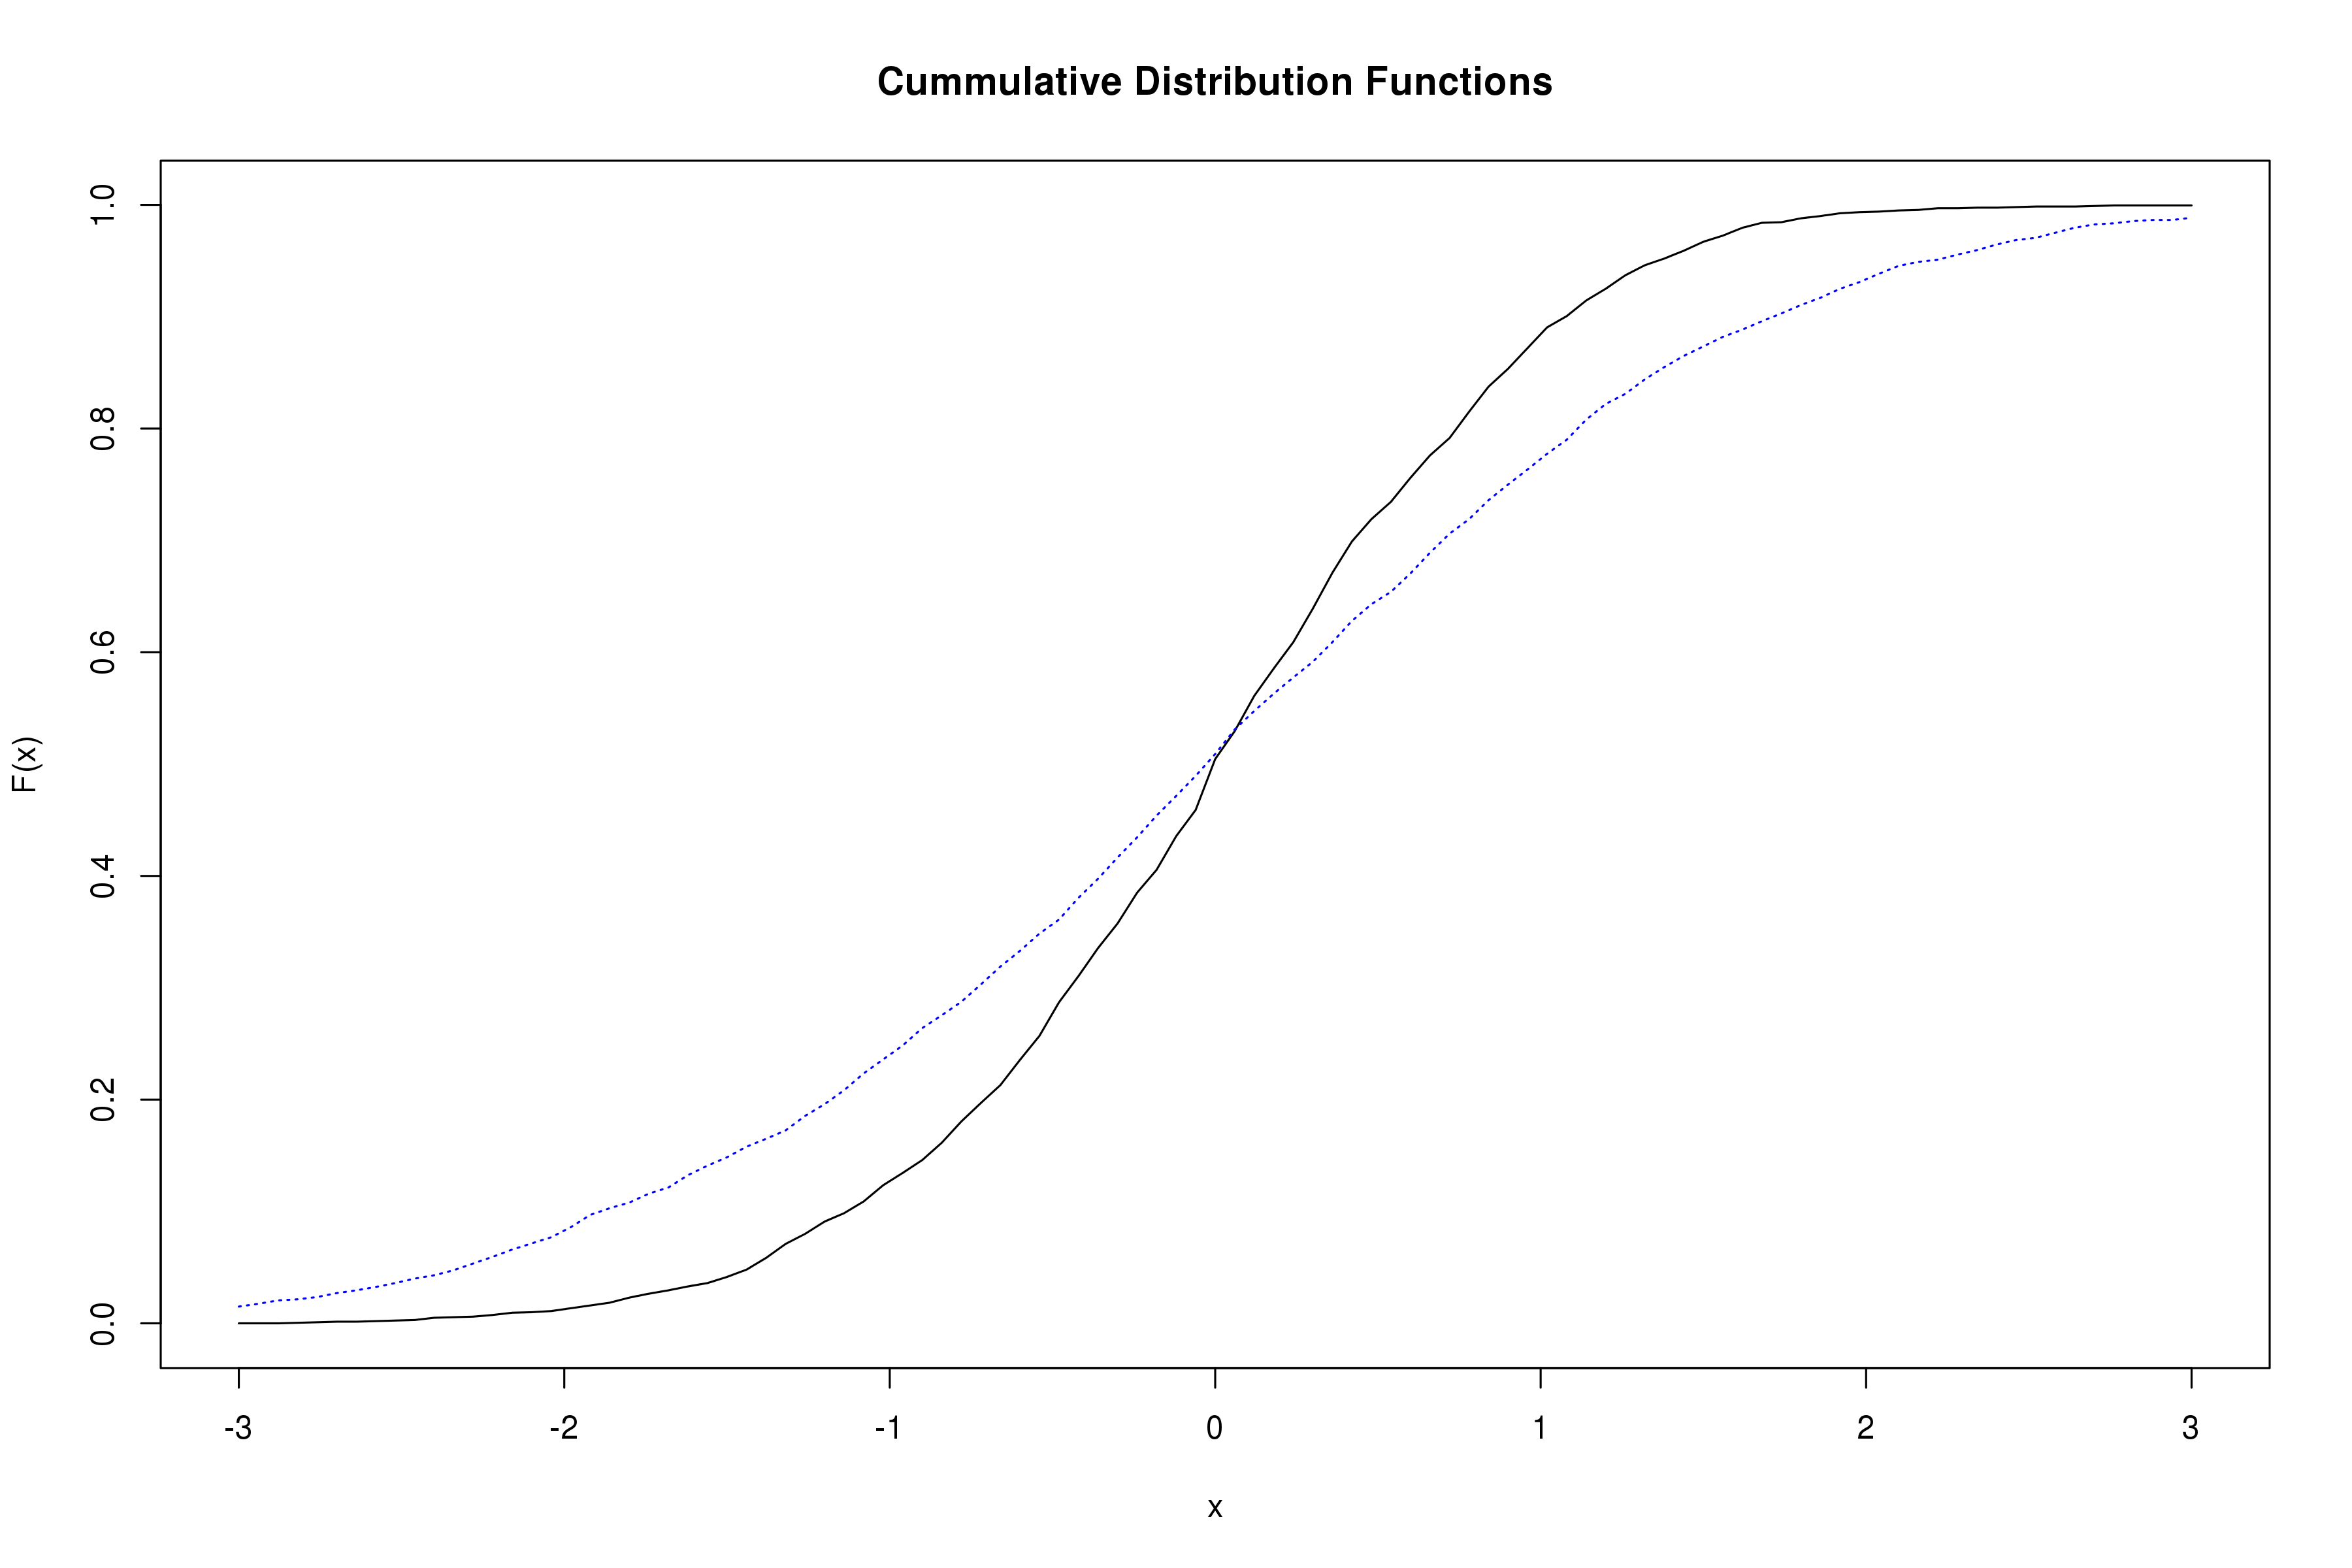
\includegraphics[width = 0.75\textwidth]{res/exA_cdf.png}
    \end{figure}
\end{frame}

